\section{Evaluation}\label{sec:eval}

A language defined by a procedure can be tested in a way no other language can: one can run the procedure and compare. We evaluate Baltmeri on three questions. Does the engine reproduce the Manual's lexicon from the Manual's rules? Does it reproduce the Manual's sentences from a grammatical analysis? And is the procedure deterministic and stable in practice?

\subsection{Reproducing the lexicon}\label{sec:eval-lex}
For each of the 58 lexical items the Manual decrees, we supplied the engine with the first dictionary translation in each of the nine languages (Appendix~\ref{app:lexicon}) and ran Algorithm~\ref{alg:synth} in the Manual's order from the initial queue. The engine reproduces \textbf{28 of 58} decrees exactly. Table~\ref{tab:rule-stats} breaks the result down by rule, and Figure~\ref{fig:rules} shows it graphically. The pattern is sharp. The Domain Rule is almost perfectly reproducible: 18 of 19 words assigned by domain come out as the Manual has them (the exception, \emph{see}, is a stem-extraction detail: Polish \emph{widzieć} gives \emph{vidz-} where the Manual takes Russian-flavoured \emph{vid-}). The Hanse Rule reproduces only 9 of 30, and the Family Vote 1 of 9.

\begin{table}[t]
\centering\small
\caption{Reproduction of the Manual's 58 lexical decrees, by the rule the engine applied.}
\label{tab:rule-stats}
\begin{tabular}{@{}lrrr@{}}
\toprule
Rule applied by engine & Decrees & Reproduced & Rate \\
\midrule
Rule 1 · Hanse & 30 & 9 & 30\% \\
Rule 2 · Domain & 19 & 18 & 95\% \\
Rule 3 · Family Vote & 9 & 1 & 11\% \\
\midrule
Total & 58 & 28 & 48\% \\
\bottomrule
\end{tabular}
\end{table}

\begin{figure}[t]
\centering
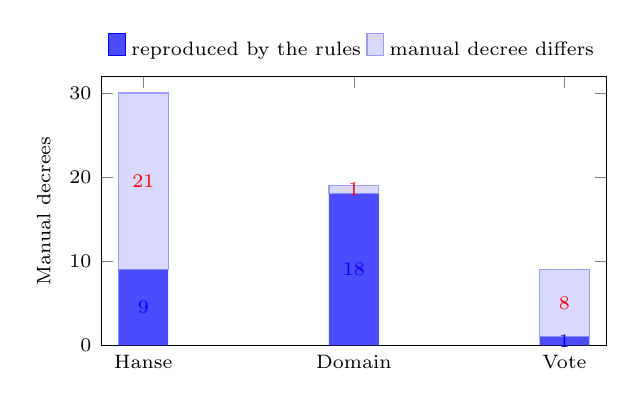
\begin{tikzpicture}
\begin{axis}[ybar stacked, width=8cm, height=5cm, bar width=18pt,
  symbolic x coords={Hanse,Domain,Vote}, xtick=data, ymin=0, ymax=32,
  ylabel={Manual decrees}, legend style={at={(0.5,1.02)},anchor=south,legend columns=2,draw=none,font=\scriptsize},
  tick label style={font=\scriptsize}, label style={font=\scriptsize}, nodes near coords, every node near coord/.append style={font=\scriptsize}]
\addplot+[fill=blue!70,draw=none] coordinates {(Hanse,9) (Domain,18) (Vote,1)};
\addplot+[fill=blue!15,draw=blue!40] coordinates {(Hanse,21) (Domain,1) (Vote,8)};
\legend{reproduced by the rules, manual decree differs}
\end{axis}
\end{tikzpicture}
\caption{Reproduction by rule. Where the Manual assigns a word by domain the engine agrees; where a word is shared or voted, the author's hand shows.}
\label{fig:rules}
\end{figure}

\paragraph{Classifying the divergences.} We read every divergent derivation trace and classified the cause (Table~\ref{tab:divergence}). Four classes account for all thirty.

\begin{enumerate}
\item \textbf{Hanse precedence (10).} The engine finds a skeleton shared by two families and inherits it; the Manual applied the Domain Rule instead. \emph{Cod}: Finnish \emph{turska}, Estonian \emph{tursk}, Swedish/Danish \emph{torsk}, Russian \emph{треска} all share T-R-S-K, so the engine takes the Hanse word (tie $\rightarrow$ Danish, \emph{torsk}); the Manual says ``Domain: Finnic (et)'' and gives \emph{tursk}. The same happens for \emph{water} (Lithuanian \emph{vanduo}, Danish \emph{vand}), \emph{winter} (Baltic \emph{ziema}, Slavic \emph{zima}), \emph{ice} (Baltic \emph{ledus}, Slavic \emph{lód}), \emph{sun} (Baltic \emph{saule}, Slavic \emph{solnce}, Germanic \emph{sol}), \emph{salmon}, \emph{cold}, \emph{sail} (Polish \emph{żeglować} is itself a Low German loan, sharing S-K-L with Swedish \emph{segla}), \emph{many} and \emph{Baltic herring}. In every case the Manual's form is the domain family's, and the domain family is Finnic nine times out of ten: the author, consciously or not, protected the sea vocabulary's Finnic character against the Hanse Rule. Whether Rule 1 or Rule 2 should have precedence for words that are both shared and domain-owned is a genuine design question the Manual's text answers one way and its examples another.
\item \textbf{Filling in a Hanse word (9).} Engine and Manual agree the word is shared and agree on the skeleton, but choose a different member's stem or a different vowel length: \emph{sild}/\emph{silk}, \emph{boot}/\emph{bot}, \emph{bu-}/\emph{buu-}, \emph{dzintar}/\emph{jantar}, \emph{tu}/\emph{du}, \emph{tri}/\emph{tre}, \emph{fem}/\emph{penki}, \emph{plav-}/\emph{pliv-}, \emph{kui}/\emph{än}. The Manual's stated procedure for this step (``family vote, ties by the Visby Queue'') underdetermines the outcome, and its own examples follow neither a whole-stem nor a position-wise vote consistently (\emph{boot} keeps the German long vowel; \emph{bu-} drops the Baltic one).
\item \textbf{Vote accounting and queue state (10).} For function words the engine's ballots or its queue state differ from the Manual's narrative. \emph{I}: the Manual counts Swedish \emph{jag} as skeleton J, discarding the final consonant, and finds J in two families; the engine reads J-K. \emph{Tomorrow}: the Manual reports a tie broken in Estonian's favour; the engine finds Germanic alone agreeing (\emph{imorgon}, \emph{i morgen}, \emph{morgen}) and lets it win outright. \emph{Question particle}: the Manual says every family abstained; the engine's one-differing-position tolerance lets Latvian \emph{vai} and Lithuanian \emph{ar} (V vs R) agree, so Baltic votes. \emph{And}: engine and Manual agree on the collision with \emph{ja} ``I'' but take a different runner-up. The remaining cases (\emph{we, you (pl.), one, no, very, but}) are of the same kind.
\item \textbf{Stem extraction (1).} \emph{See}, above.
\end{enumerate}

\begin{table}[t]
\centering\small
\caption{The thirty divergences by cause.}
\label{tab:divergence}
\begin{tabular}{@{}p{3.1cm}rp{3.7cm}@{}}
\toprule
Cause & $n$ & Items \\
\midrule
Manual applied Domain where a skeleton is shared & 10 & baltic-herring, many, water, sail, winter, ice, cod, salmon, sun, cold \\
Different fill-in of a shared skeleton & 9 & herring, boat, amber, be, you, three, five, swim, than \\
Vote accounting or queue state & 10 & I, we, you-pl, one, and, no, question, tomorrow, very, but \\
Stem extraction & 1 & see \\
\bottomrule
\end{tabular}
\end{table}

Two conclusions follow. First, the Manual is \emph{almost} an algorithm: the two rules that carry most of the semantic weight---who owns a domain, and which words are already shared---are reproduced, and the divergences sit in the last, least-specified step of filling in a shared form and in the bookkeeping of ballots. Second, the divergences are not random. They protect the Finnic character of sea vocabulary and prefer shorter, more Scandinavian-looking forms (\emph{sild} over \emph{silk}, \emph{fem} over \emph{penki}, \emph{tri} over \emph{tre}). This is exactly the editorial taste the design set out to remove, and the value of the exercise is that it can now be seen and argued about. The Manual remains authoritative for the seed lexicon (its forms are used, and the translator marks them ``manual decree''); the engine is authoritative for every word coined after it.

\paragraph{Sensitivity to the matching threshold.} The one interpretive decision with the largest effect is the length below which skeletons must match exactly (\S\ref{sec:skeleton}). Allowing one differing position at all lengths makes almost every short word a Hanse word: ``sea'' became a blend of \emph{meri}, \emph{mor} and \emph{juur} and reproduction fell to 16 of 58. Requiring exact matches for one- and two-consonant skeletons in Rule 1 raised it to 28. Extending the same restriction to family ballots in Rule 3 would fix the question particle but break \emph{many} (Latvian \emph{daudz} T-T and Lithuanian \emph{daug} T-K must agree for Baltic to vote, as the Manual says they do). We keep the Manual's wording for Rule 3 and record the tension.

\subsection{Reproducing the sentences}\label{sec:eval-sent}
We hand-wrote grammatical analyses (lemma, case, number, tense, person, order) for the Manual's twelve example sentences and the first sentence of its text, and rendered them with the engine using the seed lexicon. Twelve of thirteen come out verbatim, including all inflection, the head-final compound \emph{peleekhülje}, the copula, negation after the copula, the question particle, and every Repair the Manual illustrates (\emph{kaljuil, pospolitist, dužim, dužit, lääste, vidit, žeglisme}). The exception is \emph{bootse} ``in a boat'', which the Manual prints as \emph{bootise}: Rule 6 as the Manual states it does not insert a vowel into a two-consonant medial cluster (compare the Manual's own \emph{vidme}, \emph{vidte}), so we treat \emph{bootise} as a slip in the text rather than a rule. The full regular paradigm of \emph{vidte} (fifteen forms) and the copula (fifteen forms) are reproduced exactly; these paradigms were the decisive evidence for the boundary-sensitive formulation of epenthesis in \S\ref{sec:repair}.

\subsection{Determinism and stability}
The engine is a pure function of its inputs: 117 automated tests run on every change, covering the Normalization Table's examples, skeleton matching, citation stripping, every Repair example, the noun, adjective, pronoun and verb paradigms, the twelve sentences, reverse parsing, and the full lexicon reproduction, with the list of thirty divergences pinned so that any change in engine behaviour is visible as a test failure. The tie-break queue is an explicit, serialisable value; a derivation records the queue before and after, so any word's coining can be replayed and audited. In the deployed translator (\S\ref{sec:engine}) the derivation of new words was stable across repeated requests and across sessions by construction of the first-derivation-wins cache.
